% Chapter 4

\chapter{How do Galaxies Acquire Mass? Assembly vs. Star Formation} % Write in your own chapter title
\label{Chapter:GalGrowth}
\lhead{Chapter 4. \emph{In-situ vs. Ex-situ growth}} % Write in your own chapter title to set the page header

\section{Background}
%What is insitu and exsitu growth
%What have the previous findings been
%Why does it matter

\section{Constraining the In-Situ vs. Ex-Situ growth in \steel}
%methods and importance of constrained histories
%mass recycling
%mass return
%following populations 

\section{Incompatible \LCDM and Stellar Mass Functions}
%Cartoons and methodology
\begin{figure}[h]
	\centering
	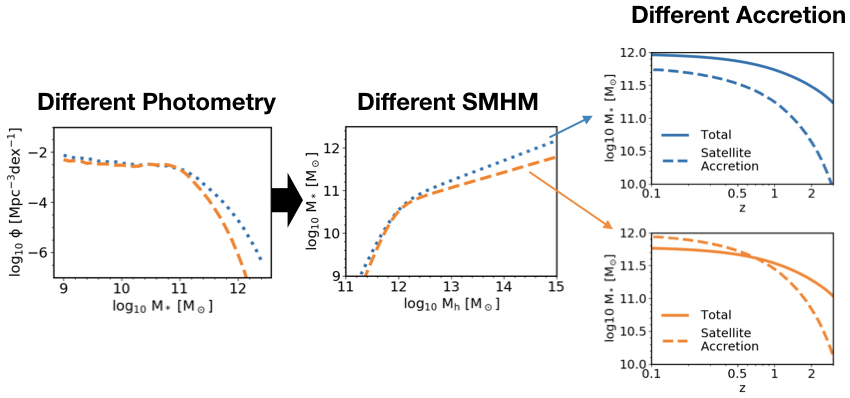
\includegraphics[width = \linewidth]{Figures/Chapter4/SMFtoAccretion.jpeg}
    \caption{}
	\label{fig:SMFtoAcc}
\end{figure}

%cmodel

\begin{figure*}
	\centering
	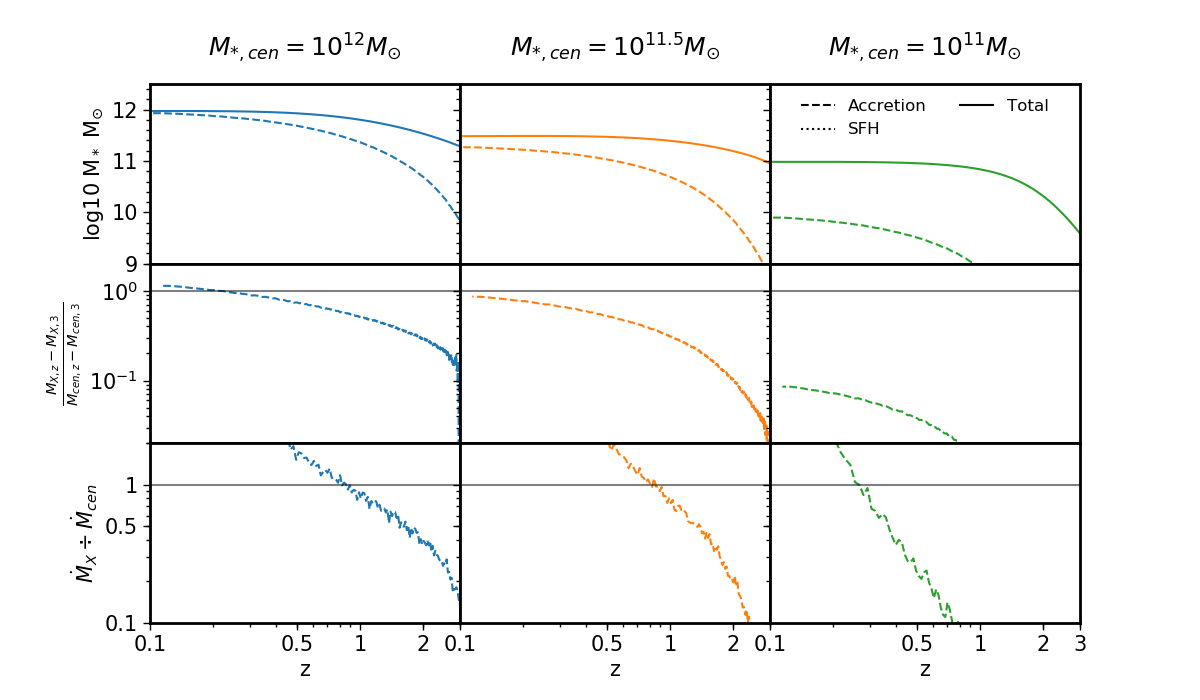
\includegraphics[width = \linewidth]{Figures/Chapter4/SatelliteAccretion_cMod.png}
    \caption{Three `mass tracks' are shown that have central galaxy masses at redshift $z = 0.1$ of $M_{*,cen}$ = $10^{12}$, $10^{11.5}$, and $10^{11}$ $[M_{\odot}]$ in blue orange and green respectively. It is clear that this model is internally nonphysical as the accretion via satellites (dashed lines) rapidly overshoots the total growth in stellar mass (solid lines) implied by the underlying growth host halo growth, as evident in the middle and bottom rows.}
	\label{fig:SatelliteAccretioncMod}
\end{figure*}

%pymorph

\begin{figure}[h]
	\centering
	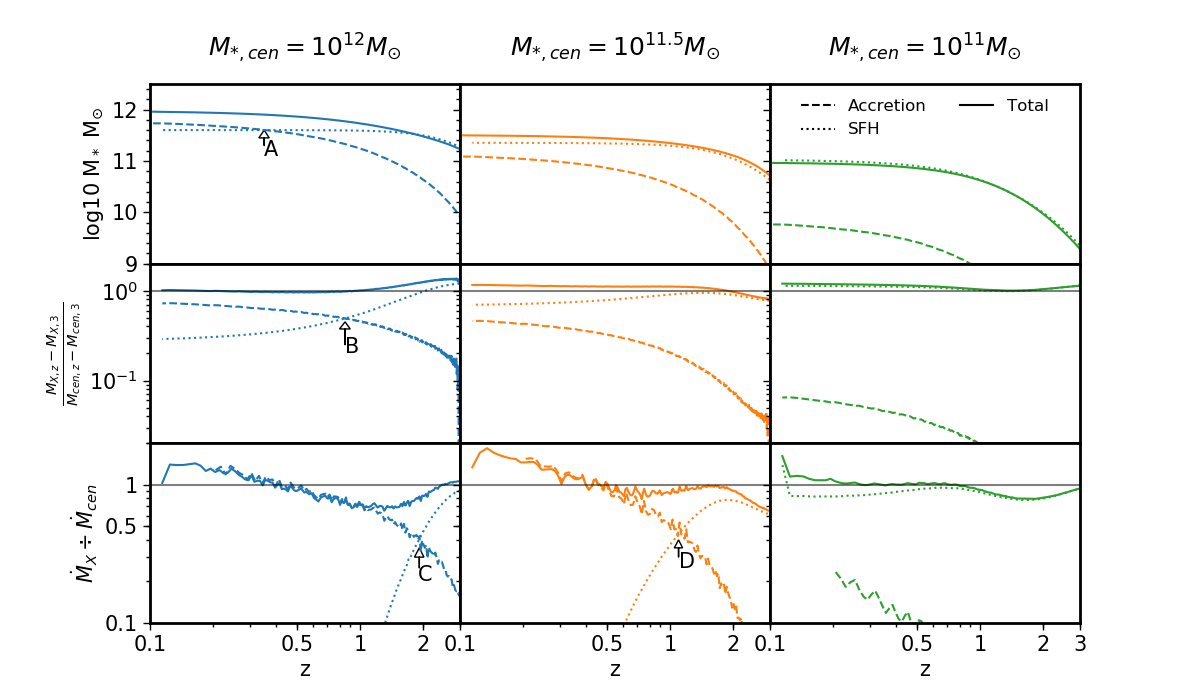
\includegraphics[width = \linewidth]{Figures/Chapter4/SatelliteAccretion_G19.png}
    \caption{Three `mass tracks' are shown that have central galaxy masses at redshift $z = 0.1$ of $M_{*,cen}$ = $10^{12}$, $10^{11.5}$, and $10^{11}$ $[M_{\odot}]$ in blue orange and green respectively. The satellite galaxy accretion is shown for evolved satellites with a dashed line, and the mass from star formation shown with a dotted line. The top panels show the total mass of the central (solid lines) and the total mass gained from accretion or star formation. The middle panels show the fraction of the total galaxy mass formed from satellite accretion or star formation since redshift $z=3$. The bottom panels show the ratio of the mass accretion rate from satellite galaxies, the star formation rate, and the mass growth rate of the central galaxy predicted by abundance matching. The black horizontal lines in the second and third rows are at unity. The solid lines showing the sum of the other two factors should be close to or on the unity lines. The labels A \& B point to where the cumulative mass from accretion overtakes the cumulative mass from star formation. The labels C \& D point to where the instantaneous accretion overtakes the star formation rate.}
	\label{fig:SatelliteAccretion}
\end{figure}

\section{Deriving the Star Formation Rate}
%Big Cartoon
\begin{figure}[h]
	\centering
	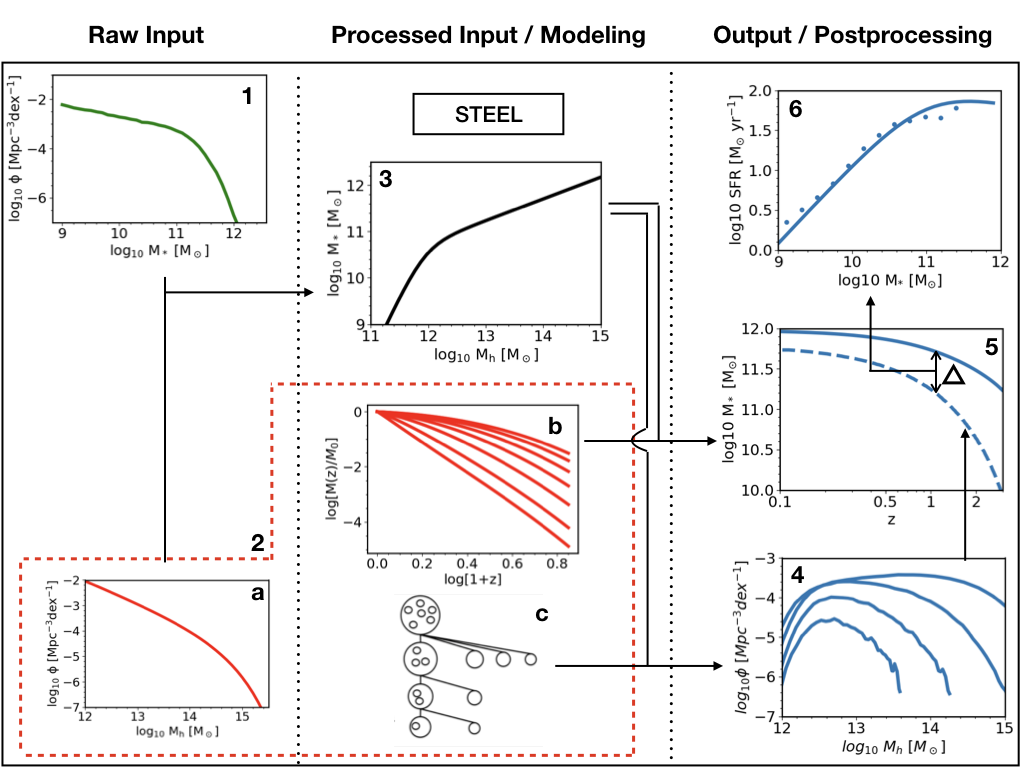
\includegraphics[width = \linewidth]{Figures/Chapter4/SFRFullCartoon.png}
    \caption{A cartoon showing the constituent steps of the method to generate star formation rates. In brief, the three columns from left to right are raw inputs, derived inputs/modelling, and output/post-processing. The subplots are: 1. The stellar mass function, 2a. The halo mass function, 2b. Halo mass growth histories, 2c. Accretion histories/Merger tree, 3. The SMHM relation, 4. Group/Cluster satellite richness, 5. Central growth histories/satellite accretion histories, 6. Star formation rate. The star formation rates are derived from the difference between the total growth in stellar mass and that from satellite accretion (panel 5).}
	\label{fig:SFRDerevation_Cartoon}
\end{figure}
%Why we cant use observed starformation rates SMF vs. SFR
%Continuity solution
%Following haloes as an improvement
\begin{figure}[h]
	\centering
	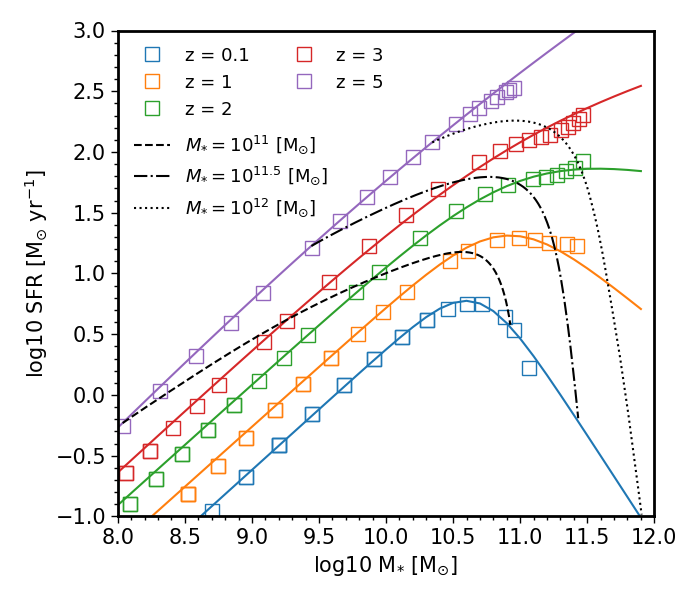
\includegraphics[width = \linewidth]{Figures/Chapter4/HMC_DPL.png}
    \caption{The star formation rate - stellar mass relation derived from following central galaxy populations along halo mass histories at redshifts $z = 0.1, 1, 2, 3, 5$. The data extracted from the post-processing of \textsc{steel} are shown by coloured crosses and the double power-law fits are shown as lines in corresponding colours. The three black lines are the evolution of the galaxy populations selected at redshift $z=0.1$ with masses $M_* = 10^{11}, 10^{11.5}, 10^{12} [M_{\odot}]$  presented in Figure \ref{fig:SatelliteAccretion}.}
	\label{fig:SFR_DPL}
\end{figure}
%Match to panchromatic data
\begin{figure}[h]
	\centering
	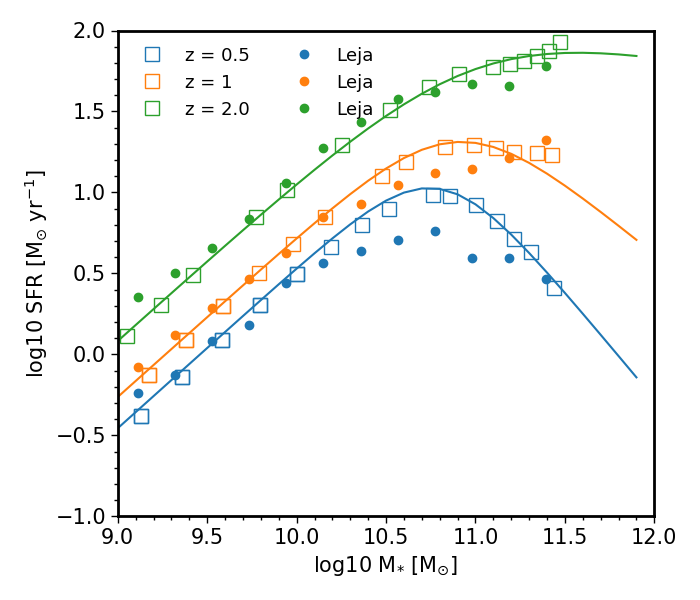
\includegraphics[width = \linewidth]{Figures/Chapter4/HMC_DPL_wLeja.png}
    \caption{I show the star formation rate - stellar mass relationship from Figure \ref{fig:SFR_DPL} at redshifts z = 0.5, 1, 2 (blue orange and green respectively, \textsc{steel} data are crosses and fits are solid lines). In this plot we compare with the observed star formation rate from \citet{Leja2018ANSURVEY} shown as filled circles with corresponding colours denoting corresponding redshift.}
	\label{fig:SFR_L18}
\end{figure}


\section{Quenching in Central and Satellite Galaxies}
%How the quenching differs
\begin{figure}[h]
	\centering
	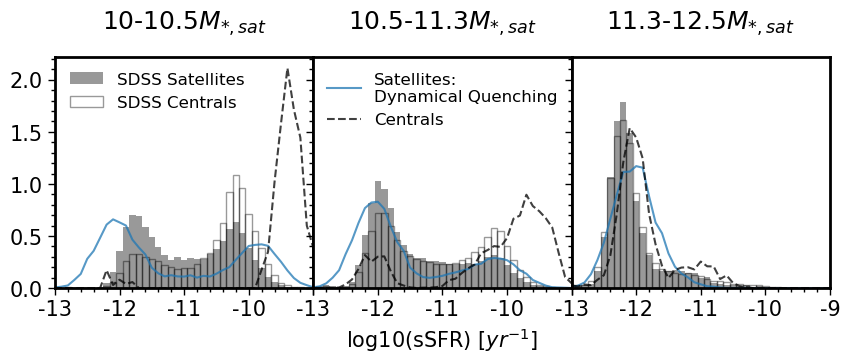
\includegraphics[width = \linewidth]{Figures/Chapter4/SSFR.png}
    \caption{I show the sSFR of satellites and centrals compared to SDSS in three mass bins selected to mirror proposed breaks in the galaxy main sequence. The SDSS data for satellites and centrals are filled and unfilled histograms respectively. The \textsc{steel} result for the satellites is the solid blue line and the post processed central result is the dashed black line.}
	\label{fig:sSFR}
\end{figure}

%what quenching is missing

%AGN probably?
